\chapter{Introducción}
\title{Introducción}
\label{cap:Introduccion}

\section{Astronomía e Instrumental Astronómico}
La astronomía es la ciencia que se ocupa del estudio de los cuerpos celestes del universo, los planetas y sus satélites, los cometas y meteoroides, las estrellas y la materia interestelar, los sistemas de materia oscura, estrellas, gas y polvo llamados galaxias y los cúmulos de galaxias, así como sus movimientos, los fenómenos ligados a ellos y las leyes que los rigen. \\

\begin{itemize}
  \item \textbf{CU-1.} Añadir una conexión.
  \begin{itemize}
    \item \textbf{Actores:} Usuario.
    \item \textbf{Tipo:} Primario, esencial.
    \item \textbf{Referencias:}
    \item \textbf{Precondición:}
    \item \textbf{Postcondición:} La nueva conexión será añadida a la lista y guardada.
    \item \textbf{Autor:} Pablo
    \item \textbf{Versión:} 1.0.
    \item \textbf{Propósito:} Añadir una nueva conexión.
    \item \textbf{Resumen:} El usuario rellenará una serie de campos y marcará unas opciones para añadir una nueva conexión a la lista.
    \end{itemize}
    \begin{table}[!ht]
      \begin{center}
	\begin{tabular}{|l|l|l|l|}
	  \hline
	  \multicolumn{4}{|c|}{{\bf Curso normal}}
	  \\ \hline
	  \multicolumn{2}{|c|}{{\bf Actor}} & \multicolumn{2}{c|}{{\bf Sistema}}
	  \\ \hline
	  {\it 1} &
	  \begin{tabular}[c]{@{}l@{}}
	    Usuario: Pulsa el botón para\\
	    añadir una nueva conexión.\\
	  \end{tabular} &
	  &
	  \\ \hline
	  &
	  &
	  {\it 2} &
	  \begin{tabular}[c]{@{}l@{}}
	    El sistema muestra el formulario\\
	    para añadir nuevas conexiones. \\
	  \end{tabular}
	  \\ \hline
	  {\it 3} &
	  \begin{tabular}[c]{@{}l@{}}
	    Usuario: Rellena los campos del \\
	    formulario, marca las opciones  \\
	    y pulsa en el botón de añadir.   \\
	  \end{tabular} &
	  &
	  \\ \hline
	  &
	  &
	  {\it 4} &
	  \begin{tabular}[c]{@{}l@{}}
	    El sistema almacena la conexión\\
	    y la añade a la lista de conexiones.\\
	  \end{tabular}
	  \\ \hline
	\end{tabular}
	\caption{CU-1. Añadir nueva conexión.}
	\label{table:cu_1}
      \end{center}
    \end{table}
\end{itemize}






\subsection{Telescopio}
El telescopio es un instrumento cuya función principal es recoger la luz de un objeto lejano y ampliarlo. Está considerado como el artífice de la astronomía moderna. \\


\begin{figure}[htb]
\centering
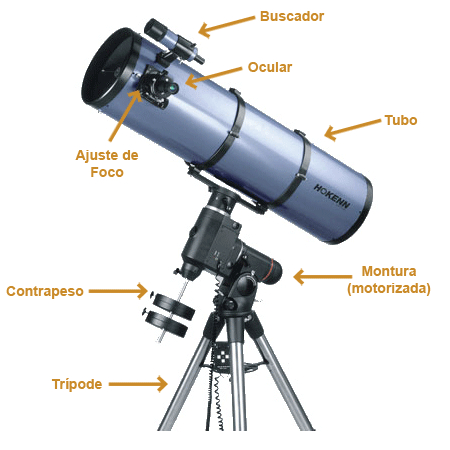
\includegraphics[width=0.6\textwidth]{./imagenes/telescopio}
\caption{Telescopio Astronómico (http://blog.astroaficion.com/)} \label{fig:telescopio}
\end{figure}
